% =========================================================================
% Hashrope: A Persistent Data Structure for Mechanisms of LLM Context
% Management  --  IEEE ICTAI submission (double-blind)
%
% BUILD (Overleaf): pdfLaTeX, main document = main.tex.
% Upload: main.tex, refs.bib, figures/*.pdf.
% HOUSE RULES: no em-dashes or en-dashes in prose; every number traces to
% a committed results file; every reference verified by web search at the
% time of addition (see refs.bib header); double-blind (no author
% identity, no artifact links until camera-ready).
% =========================================================================
\documentclass[10pt,conference]{IEEEtran}

\usepackage[T1]{fontenc}
\usepackage[utf8]{inputenc}
\usepackage{graphicx}
\usepackage{amsmath,amssymb}
\usepackage{booktabs}
\usepackage{balance}
\usepackage{url}

\graphicspath{{figures/}}

\newcommand{\hr}{\textsc{hashrope}}
\newcommand{\ms}{\,ms}
\newcommand{\us}{\,$\mu$s}

\begin{document}

\title{Hashrope: A Persistent Data Structure for Mechanisms of LLM Context
Management}

\author{\IEEEauthorblockN{Anonymous Author(s)}
\IEEEauthorblockA{Anonymous Affiliation\\
Submission to IEEE ICTAI}}

\maketitle

\begin{abstract}
Serving stacks for large language models manage context through four
recurring mechanisms: incremental edits to a growing context, branching
and snapshotting for tree search, identification of reusable prefixes for
KV-cache reuse, and encoding of repeated segments. Each mechanism is
served today by a different specialist structure. We show that all four
reduce to a single persistent weight-balanced rope whose every node
carries a polynomial hash of its subtree over a Mersenne prime, so that
the structure supports logarithmic edits and logarithmic verified
content-identity queries at the same time. We validate each mechanism
with pre-registered, replicated experiments (nine runs per point,
deterministic operation-count guards), then compare against a deployed
specialist per mechanism: the Ropey editing library, a faithful
PagedAttention copy-on-write block table, and the vendored SGLang radix
matcher. On workloads that interleave edits with identity queries, \hr{}
is net-superior to Ropey by a factor that grows without bound (369.7x at
one million characters, 9/9 paired). Against the radix matcher on a live
vLLM stack serving Qwen2.5-7B-Instruct-1M on four A100 GPUs, \hr{}
identifies a one-million-token shared prefix exactly (0 mismatches in
1800 checks, non-vacuity established by 105/105 corrupted-entry
controls) and 1.20x faster (9/9 paired, p = 0.002), at a context length
the dense engine cannot even prefill. The same experiment measures what
prefix reuse is worth on real hardware: the engine's own prefix cache
reduces GPU energy per generated token by 69.6x to 277.6x as the shared
prefix grows, a saving we attribute to the engine, with the identity
layer adding exactly zero GPU work. The structure makes verified reuse a
first-class logarithmic query instead of a linear scan.
\end{abstract}

\begin{IEEEkeywords}
persistent data structures, ropes, polynomial hashing, LLM serving,
KV-cache reuse, context management
\end{IEEEkeywords}

% =========================================================================
\section{Introduction}\label{sec:intro}

A language model serving stack spends much of its life doing string
bookkeeping. A conversation grows by appended turns and tool outputs;
an agent edits the middle of its working context; tree search forks one
context into many branches~\cite{yao2023tot}; schedulers look for
prefixes that two requests share so the KV cache of one can serve the
other~\cite{kwon2023pagedattention,zheng2024sglang,gim2024promptcache};
and system prompts, few-shot exemplars, and template headers repeat
across thousands of requests. These are four distinct mechanisms:
incremental edit, branch and snapshot, prefix-reuse identification, and
repetition encoding. In deployed systems each mechanism has its own
specialist. Text ropes handle edits~\cite{boehm1995ropes,ropey}.
PagedAttention shares KV blocks between branches through ref-counted
copy-on-write block tables~\cite{kwon2023pagedattention}. SGLang finds
reusable prefixes with a radix tree over cached token
sequences~\cite{zheng2024sglang}. Repetition is handled ad hoc, usually
by materializing the repeated bytes.

This paper makes a unification claim: all four mechanisms are served by
one structure. \hr{} is a persistent weight-balanced binary
rope~\cite{boehm1995ropes,nievergelt1973bounded} in which every node
additionally stores a polynomial fingerprint~\cite{karp1987efficient} of
the byte string its subtree represents, computed over a Mersenne prime
and maintained through every operation, in the spirit of a hash
tree~\cite{merkle1987digital} but over an editable, rebalancing
structure. Persistence~\cite{driscoll1989persistent} makes forks cheap;
the balance invariant makes edits logarithmic; and the maintained
fingerprints make content identity a logarithmic query rather than a
linear recomputation. The combination is the point. A plain rope edits
in $O(\log N)$ but answers ``do these two contexts share a prefix, and
how long is it'' only by scanning. A radix cache answers the reuse
question but is not an editable representation of the context itself. A
hash tree certifies content but is not built for splits, joins, and
rebalancing. \hr{} does all of it in one object, so the context an
agent edits, the snapshot a search forks, and the key a scheduler
matches are the same thing.

We support the claim with three layers of evidence, all pre-registered
and replicated (three seeds, three process invocations, nine runs per
point, mean and standard deviation across runs, exact paired sign
tests):

\begin{itemize}
\item \textbf{Mechanism validation} (Section~\ref{sec:mechanisms}).
Each mechanism is confirmed with a deterministic operation-count guard
plus wall-clock scaling on real corpus data: exact tokenizer-aligned
ingestion, linear-time flatten with zero hash recomputation,
$O(B\log N)$ branching memory, $O(\log^2 N)$ longest-common-prefix
queries, and $O(\log q)$ repetition encoding.
\item \textbf{Competitive studies} (Section~\ref{sec:competitive}).
One deployed specialist per mechanism: Ropey 1.6.1~\cite{ropey} for
edits (Rust against Rust), a faithful reimplementation of the
PagedAttention block-table copy-on-write
design~\cite{kwon2023pagedattention} for branching, and the vendored
SGLang RadixCache~\cite{zheng2024sglang} for identification. Wins and
losses are both reported; the losses delimit the regime where the
unification pays.
\item \textbf{Live serving-stack validation}
(Section~\ref{sec:realstack}). On vLLM with
Qwen2.5-7B-Instruct-1M~\cite{yang2025qwen1m} across four A100 GPUs,
\hr{} identifies shared prefixes exactly and, beyond a crossover length
that an independent CPU study predicted in advance, faster than the
production radix matcher, including at a one-million-token length the
dense engine cannot serve. The same runs measure the GPU energy that
prefix reuse is worth, attributed honestly to the engine's cache.
\end{itemize}

Two results preview the flavor. First, on edit-plus-identity workloads
the advantage over the editing specialist grows without bound with
context size, reaching 369.7x at one million characters and 2901.8x at
ten million, because the fingerprint is read in $O(1)$ where the
baseline must recompute it in $O(N)$. Second, the live-stack crossover
against the radix matcher falls between 524{,}288 and 1{,}000{,}000
tokens, and the prediction of an earlier CPU-only model, roughly 571k,
lands inside that bracket: a pre-registered quantitative prediction
confirmed on real serving hardware.

% =========================================================================
\section{The Hashrope Structure}\label{sec:structure}

\hr{} represents a byte string as an immutable binary tree with three
node kinds. A \emph{leaf} stores a block of bytes. An \emph{internal}
node represents the concatenation of its two children. A \emph{repeat}
node represents $q$ consecutive copies of its child. Every node stores
the length of the string it represents, its weight (leaf count), and a
polynomial hash of that string.

\textbf{Hashing.} For a byte string $S = s_0 s_1 \ldots s_{n-1}$ the
fingerprint is
$H(S) = \sum_{i=0}^{n-1} (s_i + 1)\, x^{\,n-1-i} \bmod p$
with $p = 2^{61}-1$ by default and base $x = 131$; the $+1$ offset
prevents leading-zero collisions, and Mersenne arithmetic keeps the
modular reduction to shifts and adds. Hashes compose: $H(A \Vert B) =
H(A)\, x^{|B|} + H(B) \bmod p$, so an internal node computes its hash
from its children in $O(1)$, and a repeat node computes
$H(S^q)$ through a geometric accumulator
$\Phi(q,\alpha) = \sum_{i=0}^{q-1}\alpha^i \bmod p$ evaluated by
repeated doubling in $O(\log q)$ multiplications. Every constructor
maintains these hash invariants, so the root hash of any \hr{} is the
fingerprint of the whole string at all times, and the fingerprint of a
freshly edited context costs one field read.

\textbf{Balance and edits.} The tree is kept weight-balanced in the
bounded-balance family~\cite{nievergelt1973bounded} using an Adams-style
balanced join~\cite{adams1993efficient}, which bounds height at
$O(\log w)$ for $w$ leaves. Concatenation is a balanced join; splitting
at a byte position descends one root-to-leaf path and rebuilds it,
touching $O(\log w)$ nodes; an insert is one split and two joins, a
delete two splits and one join. Because nodes are immutable, every
operation returns a new root that shares all untouched subtrees with
its input~\cite{driscoll1989persistent}: an edit allocates $O(\log w)$
nodes, and a fork allocates zero until the branches diverge.

\textbf{Substring hashes and prefix queries.} The fingerprint of any
substring is assembled from stored node hashes without materializing
bytes: a range decomposes into $O(\log w)$ fully covered subtrees,
whose stored hashes are combined by the composition rule, plus at most
two partial leaves. On top of this, the longest common prefix of two
ropes is found by binary search on prefix hashes, comparing two
substring fingerprints per step: exactly
$2\lceil\log_2 N\rceil$ hash comparisons, independent of content, for
an $O(\log^2 N)$ identity query that never scans the text.

\textbf{Byte-index contract.} The structure stores, splits, and hashes
bytes; all indices are byte offsets. Splitting UTF-8 text at an
arbitrary byte offset is exact over bytes (the halves concatenate back
to the original and all hashes are over bytes), and character-boundary
alignment is the caller's concern. Python and Rust implementations
exist; the CPU studies below use the Python implementation except the
edit study, which is Rust against Rust. We do not claim cross-language
hash byte-identity in this paper.

% =========================================================================
\section{Four Mechanisms, One Structure}\label{sec:mechanisms}

We first confirm that each mechanism behaves as the analysis says it
must, on real corpus data. Every experiment follows one protocol:
pre-registered promotion criteria written before any data; three corpus
seeds crossed with three independent process invocations (nine runs per
cell); mean and standard deviation reported across runs; and, wherever
the claim is structural, a deterministic operation-count guard whose
value is a proof rather than an estimate. Absolute Python timings carry
an interpreter constant; for those results the transferable content is
the guard-proven operation count and the measured scaling exponent, and
the Rust edit study in Section~\ref{sec:competitive} shows the direct
numbers. Table~\ref{tab:mechanisms} summarizes.

\begin{table}[t]
\caption{Mechanism validation. Guards are deterministic (std = 0);
timings are mean over 9 runs. Slopes are log-log wall-clock exponents.}
\label{tab:mechanisms}
\centering
\footnotesize
\begin{tabular}{@{}llll@{}}
\toprule
Mechanism & Bound & Guard & Headline \\
\midrule
Ingestion & exact tokens & 0 divergences & 7.6x at 16-way \\
Flatten & $O(N)$ & 0 re-hash / re-alloc & 800x vs re-split \\
Branching & $O(B\log N)$ mem & $O(\log w)$/fork & 166x at 8\,MB \\
Identify & $O(\log^2 N)$ & $2\lceil\log_2 N\rceil$ steps & slope 0.028 \\
Repetition & $O(\log q)$ & 1 node per repeat & $10^6$x at $q{=}10^4$ \\
\bottomrule
\end{tabular}
\end{table}

\textbf{Ingestion with exact token identity.} Snapping leaf boundaries
to tokenizer-safe split points lets disjoint leaves be tokenized in
parallel while reproducing the whole-string token IDs exactly: zero
boundary divergences across byte-BPE, SentencePiece, and WordPiece
families. Given that identity guarantee, chunking alone yields a stable
1.46x to 1.50x single-thread gain at 1\,MB to 4\,MB contexts, and
16-way parallelism reaches 6.62 $\pm$ 0.37 (thread pool) and 7.59
$\pm$ 0.41 (multiprocessing) on GPT-2 tokenization of 4\,MB inputs,
with multiprocessing beating threads 9/9 (p = 0.004) at a modest 13 to
16 percent margin. One honest exception: at 1\,MB with the T5
tokenizer, threads edge multiprocessing (not significant). Contexts of
256\,KB and below are overhead-dominated and excluded from claims.

\textbf{Flatten in linear time.} Materializing the rope to contiguous
bytes by in-order leaf traversal performs zero splits, zero leaf
re-allocations, and zero hash recomputations (guard), completing 2\,MB
in 0.546 $\pm$ 0.016\ms{} against 437 $\pm$ 60\ms{} for a midpoint
re-splitting strategy that re-hashes every byte, a roughly flat 730x to
800x advantage for inputs of 1\,MB and above. Both paths scale
linearly (log-log slopes 1.034 and 1.044); the eliminated cost is
redundant re-hashing, not tree depth.

\textbf{Branch and snapshot in $O(B\log N)$ memory.} Forking a context
allocates only the root-to-leaf spine when a branch first diverges. The
node-count guard is exactly deterministic: at $N = 2$\,M and $B = 50$
branches, the rope arms hold 1{,}477 unique objects against 49{,}927
for deep copies (33.8x structural sharing), with about
$\lceil\log_2 w\rceil$ new nodes per fork, matching the bound. Measured
memory compression grows with context size, reaching 166x at $N = 8$\,M
with $B = 100$ (159\,KB against 25.8\,MB), and per-fork rope memory is
near constant (slope 0.183) while deep-copy memory is linear (slope
0.884). Fork creation takes about 0.037\ms{} independent of $N$,
against 4 to 17\ms{} for deep copies (114x to 454x). This corrects an
earlier internal $O(1)$ memory intuition: the honest bound is
$O(B\log N)$, and it is what the data supports.

\textbf{Prefix-reuse identification in $O(\log^2 N)$.} The
binary-search LCP performs exactly $2\lceil\log_2 N\rceil$ hash
comparisons at every size (guard), and wall clock corroborates the
bound with a log-log slope of 0.028 across 64\,KB to 8\,MB, against
1.008 for byte-by-byte comparison; the crossover with the byte scan
falls near 1\,MB. At 8\,MB the hash LCP completes in 19\ms{} wherever
the divergence lies, against 99 to 200\ms{} for scanning. Correctness
is exact: zero mismatches against a byte-level oracle in 162 checks.
A dedup workload with ten prompts sharing a 1.2\,MB prefix identifies
the shared prefix for 98.5 percent of pairs at 20.9\ms{} per pair.

\textbf{Repetition in $O(\log q)$.} Encoding $q$ copies of a unit
creates one repeat node wrapping the unit subtree and computes the hash
through the geometric accumulator. At $q = 10^4$ with a 4\,KB unit,
that is 2 objects, 327 bytes, and 11\us{} to represent 40\,MB of
logical content, against 19{,}999 nodes, 44\,MB, and 10.6\,s for naive
materialization: a node compression near $10^4$ and a construction
speedup near $10^6$, with construction slopes 0.175 (repeat) against
1.041 (naive). A unit-size sweep separates the two costs: naive
construction grows linearly with unit length, while the repeat-node
cost stays near 0.01\ms{} regardless of the unit. Repeated system
prompts, few-shot exemplars, and template headers are encoded once.

% =========================================================================
\section{Against the Specialists}\label{sec:competitive}

Unification is only interesting if the unified structure is competitive
with the specialist on each specialist's home ground, and clearly
better once identity enters the workload. We test one deployed
implementation per mechanism. Setup is never timed; only the operation
under test is. All comparisons are paired on identical seeded
workloads.

\textbf{Edits: against Ropey (Rust against Rust).} Ropey
1.6.1~\cite{ropey} is a production text rope used by editors. We vendor
it (pinned, checksum verified) and drive both arms with one seeded
churn sequence (delete a random span, insert an equal-length span) on
ASCII buffers so character and byte indices coincide. \hr{} maintains
its fingerprint eagerly on every edit; Ropey, which maintains no hash,
is given \hr{}'s own polynomial hash to run over its materialized bytes
when identity is queried, so the comparison is maintained-incrementally
against recomputed-from-scratch with the same hash function. Two
findings. On raw churn, both arms are in the same $O(\log N)$ class
(per-edit slopes 0.202 against 0.212); \hr{} pays a bounded constant
factor for the maintained fingerprint that peaks at 22.0x near 100\,K
and declines to 14.0x at 10\,M as both arms go logarithmic. On the
workload that motivates a content-indexed structure, cycles of edits
followed by a whole-buffer identity query, \hr{} wins at every size and
the advantage grows without bound: 3.0x at 1\,K, 47.6x at 100\,K,
369.7x at 1\,M (9/9 paired, p = 0.0039), 2901.8x at 10\,M
(Fig.~\ref{fig:editidentity}). The mechanism is visible in the
per-cycle slopes: 1.013 for Ropey (the $O(N)$ recompute dominates)
against 0.150 for \hr{} (an $O(1)$ fingerprint read plus logarithmic
edits). Because that argument depends on how often identity is
queried, we ablate the query-to-edit ratio $r$
(Table~\ref{tab:rsweep}). The crossover moves outward exactly as the
cost model predicts, from 1\,K characters at one query per cycle to
300\,K at one query per hundred cycles, and below each crossover Ropey
wins (down to 0.2x at small $N$ under $r = 0.01$), an honest negative
that delimits the regime. Above the crossover \hr{} wins 9/9 at every
size, and even at $r = 0.01$ the advantage reaches 27.7x at 10\,M,
because Ropey's per-cycle slope stays near one at every ratio (1.013,
1.007, 0.943) while \hr{}'s stays near 0.2. One more honest cost:
persistence retains dead path nodes under in-place-style churn, about
2.7 additional retained nodes per doubling of $N$, the flip side of
the immutability that makes forks free.

\begin{table}[t]
\caption{Query-to-edit ratio ablation against Ropey: per-cycle speedup
(Ropey over \hr{}), nine runs per point, 9/9 paired at and above each
crossover $N^{*}$. Below $N^{*}$ Ropey wins.}
\label{tab:rsweep}
\centering
\footnotesize
\begin{tabular}{@{}lrrrr@{}}
\toprule
$r$ (queries/cycle) & $N^{*}$ & 100\,K & 1\,M & 10\,M \\
\midrule
1    & 1\,K   & 47.6x & 369.7x & 2901.8x \\
0.1  & 10\,K  & 5.3x  & 32.2x  & 265.0x \\
0.01 & 300\,K & 0.7x  & 3.8x   & 27.7x \\
\bottomrule
\end{tabular}
\end{table}

\begin{figure}[t]
\centering
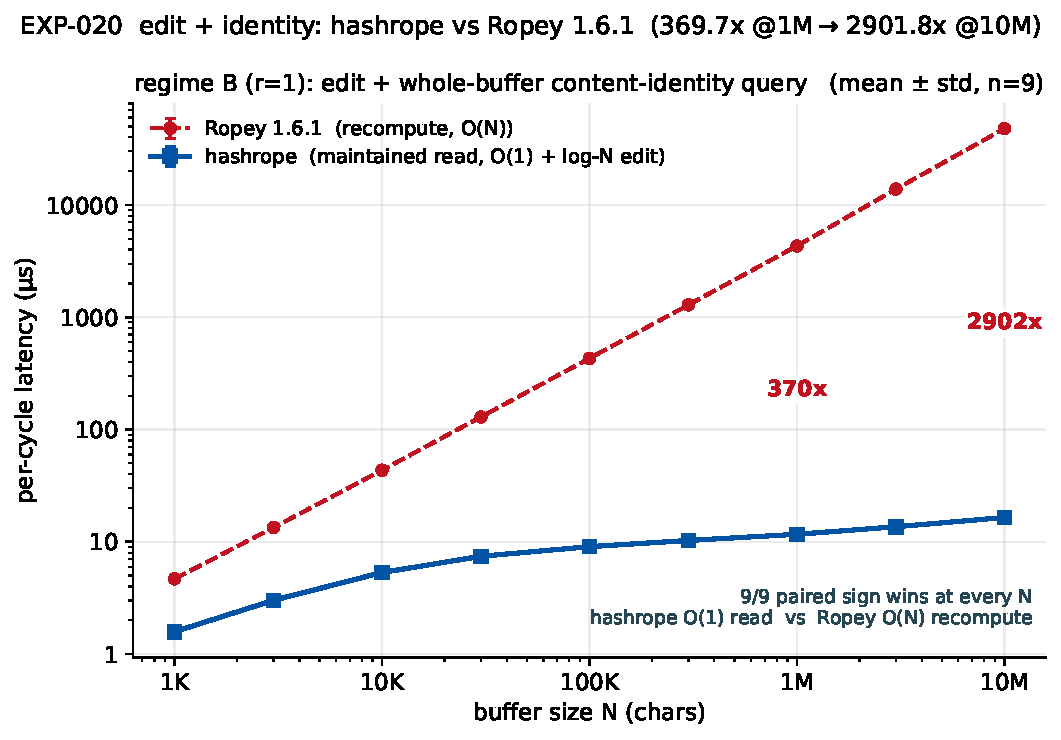
\includegraphics[width=\columnwidth]{exp020_edit_identity_latency}
\caption{Edit-plus-identity workload, \hr{} (Rust) against Ropey 1.6.1
with the same polynomial hash: per-cycle latency over buffer size, nine
runs per point. Ropey's cycle is dominated by the $O(N)$ fingerprint
recompute (slope 1.013); \hr{} reads the maintained fingerprint in
$O(1)$ (slope 0.150), so the gap widens without bound: 369.7x at 1\,M
characters, 2901.8x at 10\,M, 9/9 paired at every size.}
\label{fig:editidentity}
\end{figure}

\textbf{Branching: against PagedAttention copy-on-write.} We
reimplement the block-table copy-on-write design of
PagedAttention~\cite{kwon2023pagedattention} faithfully (ref-counted
physical blocks, per-sequence block tables, copy-on-write fork and
append; 55 unit tests) and compare branch creation, defined as fork
plus the first divergent step so that \hr{} is charged its full
$O(\log w)$ spine. \hr{} branch creation is essentially flat, 26\us{}
to 37\us{} from 1\,K to 1\,M tokens, while the block table scales as
$O(\lceil N/B\rceil)$, reaching 3.6\ms{} at 1\,M with block size 16:
crossover at 16\,K tokens for the reference block size, 97.4x at 1\,M
(168.7x at block size 8), 9/9 paired at every block size. Holding five
branches of a 1\,M-token context costs \hr{} about 9.2\,KB against
5.63\,MB for the paged table at block size 8 (613x; 306x at block 16),
because the table is $\Theta(N/B)$ per branch while \hr{} adds only the
shared logarithmic spine (Fig.~\ref{fig:branchmem}). Both sides carry
deterministic guards at every cell: \hr{} allocates at most
$\lceil\log_2 w\rceil + 3$ new nodes per branch, and the baseline's
fork copies exactly the block-table entries the design specifies. A
branch-count ablation over $B \in \{5, 10, 25, 50\}$ shows the
compression is invariant to beam width, rising slightly from 613x to
639x at block size 8 as $B$ grows (both sides scale linearly in $B$);
fifty branches of a 1\,M-token context fit in 86\,KB against
53.7\,MB. An ecological replay corroborates the controlled sweep with
real search: tree-of-thought traces~\cite{yao2023tot} generated by a
120B open-weight model on Game of 24 (75 trees, 7{,}943 nodes,
7{,}868 branch creations at beam 5, depth 3), recorded once and
replayed deterministically through the same harness over prompt
prefixes up to 256\,K tokens. Every node context reconstructs
byte-identically in both arms (0 mismatches at every prefix and block
size), \hr{} branch creation stays flat at 16\us{} to 24\us{} while
the paged table reaches 1.82\ms{}, giving 74.6x, 38.9x, 19.1x, and
9.6x at the 256\,K prefix for block sizes 8 through 64 (9/9 paired at
every block size), and marginal branching memory on the real
five-survivor beams compresses 17x to 67x across the
deployment-standard block sizes. Below the 16\,K crossover the paged
table is faster, as expected for short contexts.

\begin{figure}[t]
\centering
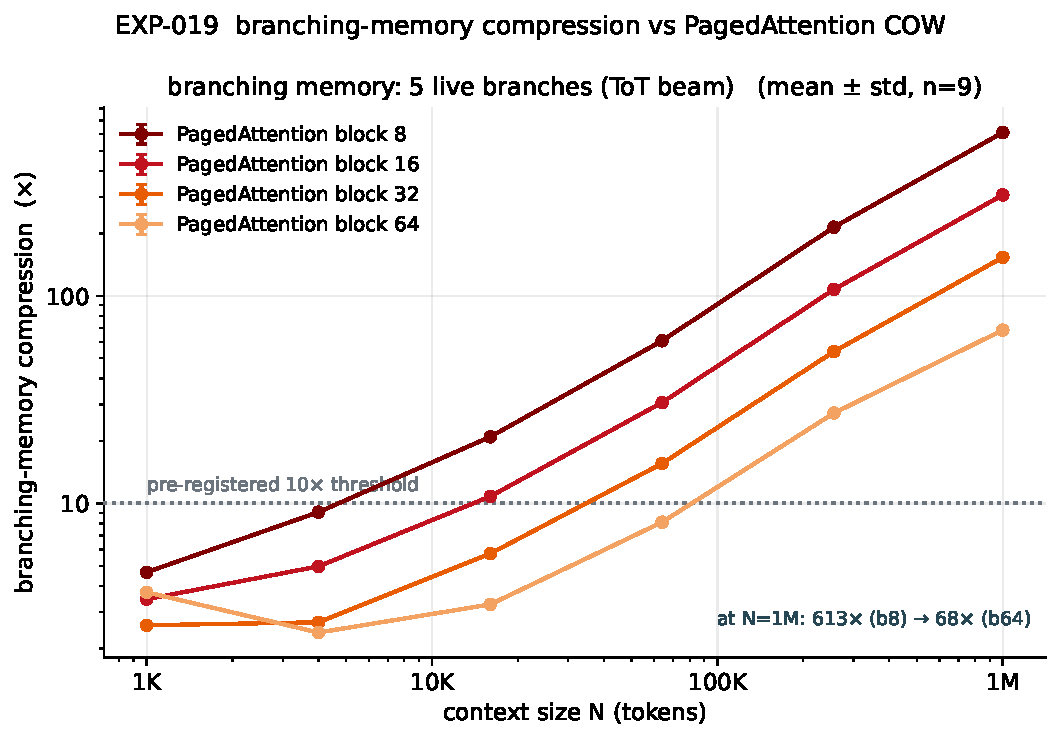
\includegraphics[width=\columnwidth]{exp019_branch_memory_compression}
\caption{Branch memory against a faithful PagedAttention block-table
copy-on-write baseline, five branches per context. The paged table is
$\Theta(N/B)$ per branch; \hr{} adds an $O(\log w)$ shared spine per
branch, so compression grows with context size (306x at 1\,M tokens at
the reference block size 16, 613x at block size 8).}
\label{fig:branchmem}
\end{figure}

\textbf{Identification: against the SGLang radix matcher.} We vendor
the RadixCache of SGLang~\cite{zheng2024sglang} byte-identically
(v0.1.17, checksum verified) and compare single-query prefix
identification over token sequences, with a NumPy flat scan as the
C-speed floor. The radix walk is $\Theta(L)$ at about 29\,ns per token;
the \hr{} LCP is near flat at 13\ms{} to 18\ms{}
(Table~\ref{tab:radix}). The crossover on CPU
falls near $L^* \approx 571$\,K tokens: 1.70x at 1\,M and 4.63x at
2\,M (9/9 paired, p = 0.004), with the advantage growing linearly in
$L$ beyond.

\begin{table}[t]
\caption{Single-query prefix identification against the vendored
SGLang radix matcher over shared-prefix length $L$ (tokens), mean over
nine runs; the flat scan is the $O(L)$ floor. Crossover near 571\,K.}
\label{tab:radix}
\centering
\footnotesize
\begin{tabular}{@{}rrrrr@{}}
\toprule
$L$ & radix (ms) & \hr{} (ms) & flat (ms) & speedup \\
\midrule
1\,K   & 0.034  & 17.83 & 0.003 & 0.00x \\
4\,K   & 0.118  & 17.77 & 0.003 & 0.01x \\
16\,K  & 0.462  & 14.32 & 0.006 & 0.03x \\
64\,K  & 2.24   & 13.07 & 0.018 & 0.17x \\
128\,K & 3.82   & 15.57 & 0.038 & 0.25x \\
256\,K & 7.47   & 15.53 & 0.082 & 0.48x \\
512\,K & 15.09  & 15.95 & 0.171 & 0.95x \\
1\,M   & 29.23  & 17.23 & 0.404 & 1.70x \\
2\,M   & 58.76  & 12.70 & 1.646 & 4.63x \\
\bottomrule
\end{tabular}
\end{table}

Two honest negatives delimit the regime. On real
conversation pairs from ShareGPT~\cite{sharegpt} and
LMSYS-Chat-1M~\cite{zheng2024lmsyschat}, whose shared prefixes average
about 2\,K tokens, the radix matcher wins every cell by orders of
magnitude (0.03\ms{} against 8.8\ms{}), and in a one-against-$K$ sweep
the radix tree answers all $K$ candidates in one walk while \hr{} pays
$K$ pairwise queries (610x to the radix side at $K = 100$). The radix
structure also requires the $O(N)$ materialized token sequence per
cached context, where \hr{} holds the compressed persistent form
(Section~\ref{sec:mechanisms}); the identification advantage claimed
here is for long shared prefixes, one pair at a time.

% =========================================================================
\section{Validation on a Live 7B Serving Stack}\label{sec:realstack}

The CPU studies leave one question open: does any of this survive
contact with a real serving engine, at lengths that matter, with
correctness verified end to end and energy measured rather than
asserted? We answer it on vLLM 0.8.5 serving
Qwen2.5-7B-Instruct-1M~\cite{yang2025qwen1m} with tensor parallelism
across four A100-40GB GPUs.

\textbf{Design.} Two decoupled tracks share every run. Track A varies
exactly one engine knob, the prefix cache (off, on), and measures GPU
energy through NVML on-board energy counters, time to first token, and
throughput. Track B runs the three identification arms (\hr{}, the
vendored radix matcher, the flat scan) on CPU, strictly outside the GPU
measurement window, over the same token streams the engine serves, so
the identity layer can never contaminate the energy measurement: with
one engine execution per cell, the difference in dispatched GPU work
between identifier arms is identically zero, and identity-layer energy
neutrality holds by construction. Two regimes: realistic multi-turn
streams drawn from ShareGPT and LMSYS-Chat-1M (median shared prefixes
near 642 tokens), and a controlled sweep of a single shared prefix of
length $L$ in $\{$131{,}072; 262{,}144; 393{,}216; 524{,}288;
1{,}000{,}000$\}$ tokens followed by short divergent queries. Nine runs
per point as before.

\textbf{Exactness, made non-vacuous.} Across every cell and seed, the
reuse prefix selected by \hr{}, the radix matcher, and the flat scan is
token-identical: 0 mismatches in 1800 checks. A gate that trivially
agreed would also score zero, so we corrupt cached entries on purpose:
a single token flipped at the first, middle, or last position of the
cached prefix, 105 controls in all, including position 999{,}999 of a
1{,}000{,}000-token prefix. Every arm detects every corruption at the
exact position, 105/105. Verified reuse here means verified. The
realistic streams also reproduce the short-prefix negative on the live
stack: at their roughly 642-token median prefixes the radix matcher
identifies in 0.037 $\pm$ 0.002\ms{} against 17.46 $\pm$ 0.91\ms{} for
\hr{} (flat scan 0.005\ms{}), consistent with the CPU study and
reported in full. Two measurement notes for reproducibility. The
engine's offline API exposes no per-request cached-token counter in
this version, so the tie between identified prefixes and actual engine
reuse is carried by the time-to-first-token and energy deltas together
with the correctness gate, not by a counter. And energy per token
divides total GPU Joules by generated completion tokens, so absolute
values are prefill-dominated; the cache-off over cache-on ratio and
the paired delta are the meaningful quantities, and they are what we
report.

\textbf{The crossover, confirmed on live hardware.} The CPU study of
Section~\ref{sec:competitive} predicted a crossover near 571\,K tokens
before any serving run. On the live stack the prediction holds:
the radix matcher is still faster at $L = 524{,}288$ (31.73 $\pm$
4.64\ms{} against 45.66 $\pm$ 0.76\ms{}) and \hr{} is faster at
$L = 1{,}000{,}000$ (44.42 $\pm$ 0.63\ms{} against 53.19 $\pm$
3.78\ms{}; 1.20x, 9/9 paired, one-sided p = 0.002), bracketing the
live-stack crossover inside the predicted region
(Fig.~\ref{fig:crossover}). \hr{}'s latency is flat across the entire
sweep, the logarithmic signature, while the radix walk grows linearly.
The one-million-token point deserves emphasis: at that length the
dense-attention engine cannot complete a prefill at all in this
configuration (the runs record the serving wall explicitly and skip
the engine track there), yet the identity layer keeps answering in
44\ms{}, which is 0.048 percent of the full prefill time at the
largest length the engine does serve. The serving wall belongs to the
engine configuration; the identification does not share it.

\begin{figure}[t]
\centering
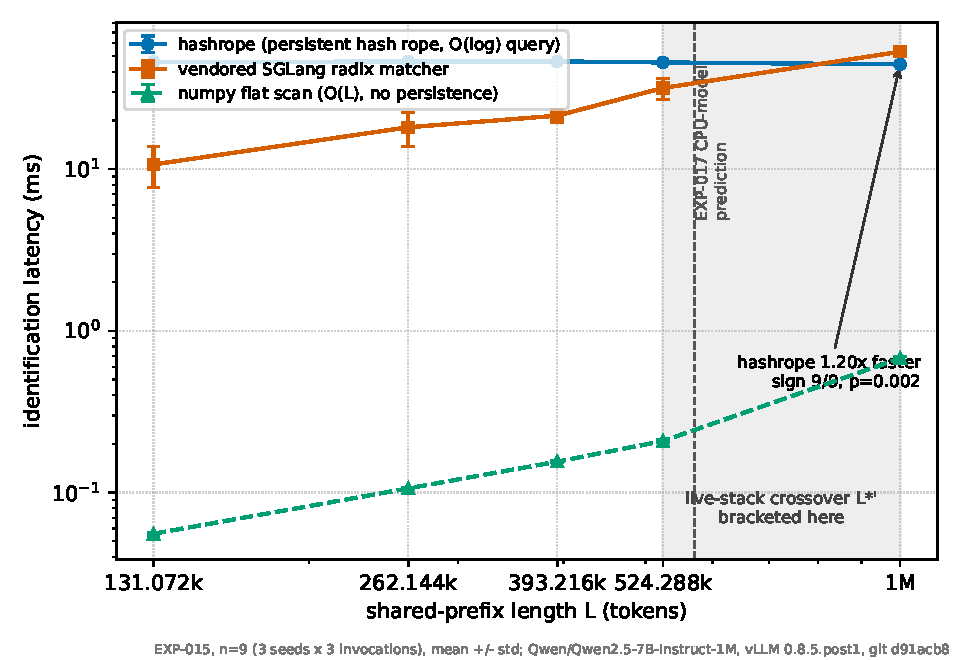
\includegraphics[width=\columnwidth]{exp015_identification_latency_vs_L}
\caption{Identification latency on the live stack over shared-prefix
length, log-log, nine runs per point. \hr{} is flat across the sweep
(the $O(\log)$ signature), the production radix matcher grows, and the
flat $O(L)$ scan has slope near one. The live-stack crossover is
bracketed between 524{,}288 and 1{,}000{,}000 tokens; the dashed line
is the crossover predicted in advance by the CPU-only study, which
lands inside the bracket. At one million tokens, a length the dense
engine cannot prefill, \hr{} beats the radix matcher 1.20x, 9/9
paired, p = 0.002.}
\label{fig:crossover}
\end{figure}

\textbf{What reuse is worth, attributed honestly.} With the cache on,
the engine's own prefix caching reduces GPU energy per generated token
by 22.65x $\pm$ 1.84 on the realistic streams and by 69.6x, 150.4x,
217.6x, and 277.6x at $L$ from 131\,K to 524\,K on the controlled
sweep, monotone in $L$, 9/9 paired with p = 0.002 at every point; time
to first token falls from 92.5\,s to 0.87\,s at $L = 524{,}288$, with
zero cache-on regressions anywhere (Fig.~\ref{fig:energy}). One
sentence of attribution matters more than any of these numbers: the
reduction is the effect of the engine's cache, not of \hr{}. What
\hr{} contributes is the verified identification that decides reuse,
at exactly zero additional GPU work and at millisecond latencies that
are a rounding error against prefill. An upstream identity layer is
redundant inside a single engine that already radix-matches its own
cache; the measured stakes say what verified identification is worth
in the settings where the engine's matcher does not reach: routing
across engine instances, cross-request deduplication, and contexts
held as opaque compressed blobs.

\begin{figure}[t]
\centering
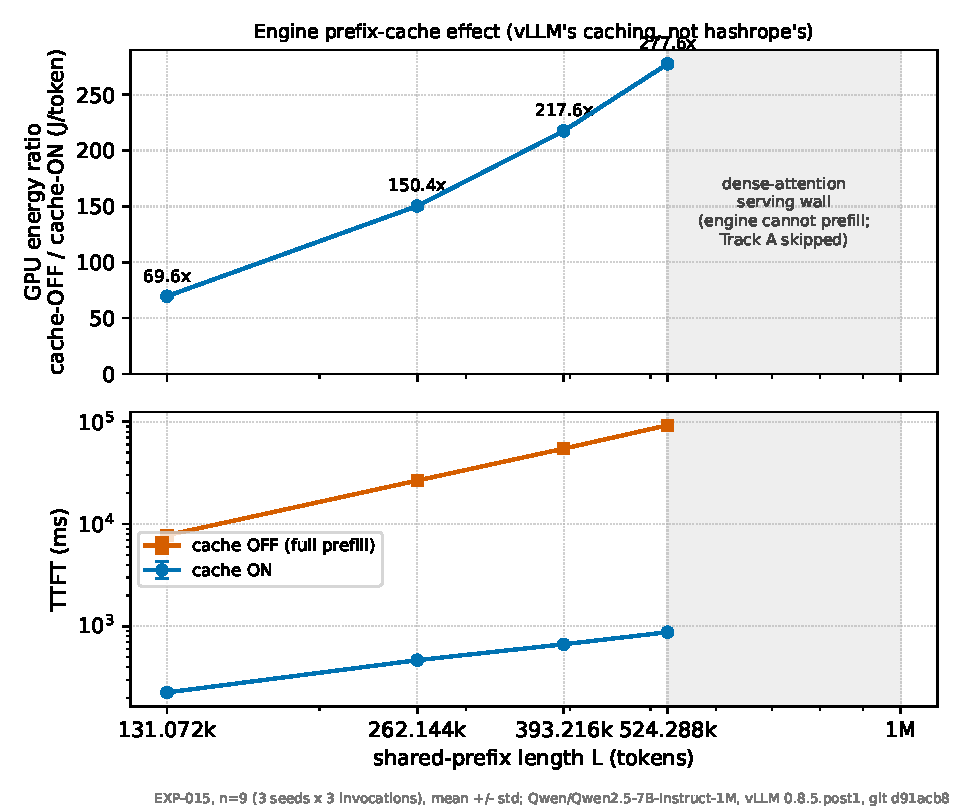
\includegraphics[width=\columnwidth]{exp015_caching_energy_vs_L}
\caption{The engine prefix-cache effect on the live stack (top: GPU
energy per generated token, cache off over cache on; bottom: time to
first token), nine runs per point. The reduction, 69.6x to 277.6x
across the sweep, is attributed to the vLLM cache, not to \hr{}; the
identity layer adds exactly zero GPU work by construction. The shaded
region marks the dense-attention serving wall, beyond which the engine
cannot prefill; identification (Fig.~\ref{fig:crossover}) keeps
working there.}
\label{fig:energy}
\end{figure}

% =========================================================================
\section{Limitations and Disclosures}\label{sec:limits}

Four limits bound the claims. First, the polynomial fingerprint uses
public parameters, so an adversary who controls content can forge
collisions; identity here is an integrity check against accidental
divergence, not an adversarial guarantee. Keyed hashing or
verify-on-match (compare bytes only when fingerprints agree) closes the
gap and is future work. Second, the identity layer is conditional on
use: inside a single engine that already maintains its own radix cache
it is redundant, and the short-prefix and one-against-many regimes
belong to the radix matcher (Section~\ref{sec:competitive}); the value
concentrates on long shared prefixes and on settings outside a single
engine's cache. Third, absolute multipliers from the Python CPU studies
carry an interpreter constant; the transferable content there is the
deterministic operation counts and the measured scaling exponents, and
the Rust edit study gives direct numbers. Fourth, the one-million-token
serving wall is a property of the dense-attention engine configuration
we measured, not of the structure, and generation quality at extreme
lengths was not scored; the engine-side claims are timing and energy
only. We also do not claim byte-identical hashes across the Python and
Rust implementations, and a per-seed provenance gap in two of the three
synthetic base contexts is documented in the project record (the
recorded corpus hashes are authoritative; results are unaffected).

% =========================================================================
\section{Related Work}\label{sec:related}

Ropes were introduced as heavyweight strings with logarithmic
concatenation and substring operations~\cite{boehm1995ropes}, and
production descendants such as Ropey~\cite{ropey} remain the editing
specialist. Weight-balanced trees~\cite{nievergelt1973bounded} and the
balanced join~\cite{adams1993efficient} supply the balancing scheme;
persistence with structural sharing follows the classical
treatment~\cite{driscoll1989persistent}. Rolling and polynomial
fingerprints originate with randomized pattern
matching~\cite{karp1987efficient}, and per-node hashes over trees with
Merkle's construction~\cite{merkle1987digital}; \hr{} carries a
Karp-Rabin-style fingerprint at every node of a rebalancing, editable
rope, which is the combination the four mechanisms need. On the
serving side, PagedAttention~\cite{kwon2023pagedattention} shares KV
blocks through paged copy-on-write tables, SGLang's
RadixAttention~\cite{zheng2024sglang} matches reusable prefixes in a
radix tree over cached tokens, and Prompt
Cache~\cite{gim2024promptcache} reuses attention states of declared
prompt modules. These systems reuse KV state given a match; \hr{}
addresses the representation question underneath them: one persistent
object that is simultaneously the editable context, the forkable
snapshot, and a verifiable content key. Tree-of-thought
search~\cite{yao2023tot} supplies the branching workload, and
ShareGPT~\cite{sharegpt} with LMSYS-Chat-1M~\cite{zheng2024lmsyschat}
the realistic conversation streams.

% =========================================================================
\section{Conclusion}\label{sec:conclusion}

Four mechanisms of LLM context management, incremental edit, branch
and snapshot, prefix-reuse identification, and repetition encoding,
reduce to one persistent weight-balanced rope with per-node polynomial
fingerprints. The structure edits and answers verified identity
queries in logarithmic time at once, holds its own against a deployed
specialist on each mechanism's home ground, dominates once identity
enters the workload, and, on a live 7B serving stack, identifies a
one-million-token shared prefix exactly and faster than the production
matcher at a length the dense engine cannot serve, while the measured
engine-side energy quantifies what such reuse is worth. Future work:
keyed or verify-on-match hashing for adversarial settings, a paired
CPU-energy study of logarithmic edits against linear copies, and
integration of the identity layer into multi-instance routing.
Implementations and the full experimental record will be released with
the camera-ready version.

\balance
\bibliographystyle{IEEEtran}
\bibliography{refs}

\end{document}
